Para la validación del proyecto se ha distribuido el paquete de herramientas a varios equipos de desarrollo con el fin de encuestar a los distintos miembros acerca de la facilidad de uso, utilidad y escalabilidad.
 Entre estos equipos se encuentran los desarrolladores de Co-Fi Space\cite{CoFiSpace}, un videojuego de 'Game Jam' y EcoRescue\cite{EcoRescue} un trabajo de fin de grado, además de una serie de agentes 
 independientes que han prestado su tiempo a probar la librería en prototipos menores.

\section{Encuestas}

De cara a validar el proyecto, la primera fuente de datos planteada fue preparar una encuesta (Disponible en el Anexo \ref{sec:apendice}) con la que obtener sensaciones e impresiones de primera mano de los equipos
 de desarrollo y agentes individuales. El objetivo de estas preguntas es tanto obtener una idea general de si la 'suite' de herramientas es verdaderamente útil e intuitivo como si realmente es escalable como
 se pretendía en un principio.

\section{Experiencia de Validación}
La experiencia en general ha sido muy buena, el feedback ha sido en su mayoría positivo o en su defecto muy útil para seguir mejorando el proyecto a futuro. Los dos juegos que han resultado a raíz del proyecto 
tienen una calidad y acabado muy altos. Los encuestados se han mostrado en todo momento muy receptivos a participar en el proceso de explicación de los componentes de la librería, comunicando su opinión y 
proporcionando feedback significativo en todo momento. Finalmente se han encuestado a catorce usuarios de la librería entre los equipos de desarrollo y encuestados independientes.

\section{Resultados Cuantitativos}
En cuanto a la discusión de resultados, se pueden observar varios patrones muy evidentes, el primero y el más importante es que, en su grandísima mayoría (ver figuras en Apéndice \ref{sec:apendice}) los encuestados
se han mostrado positivos al ser preguntados acerca de la facilidad de uso e implementación de cada uno de los componentes o sistemas de la librería. Una notable excepción es la del generador de mazmorras, donde
 casi un 30\% (Figura \ref{fig:CUESTIONARIO_14trucado}) de los encuestados se han mostrado parcialmente o completamente en desacuerdo con que sea un sistema sencillo de utilizar, cabe destacar que esto es algo que 
 también se ha mencionado como feedback adicional (Figura \ref{fig:tablaFeedback}).

\begin{figure}[H]
  \centering
  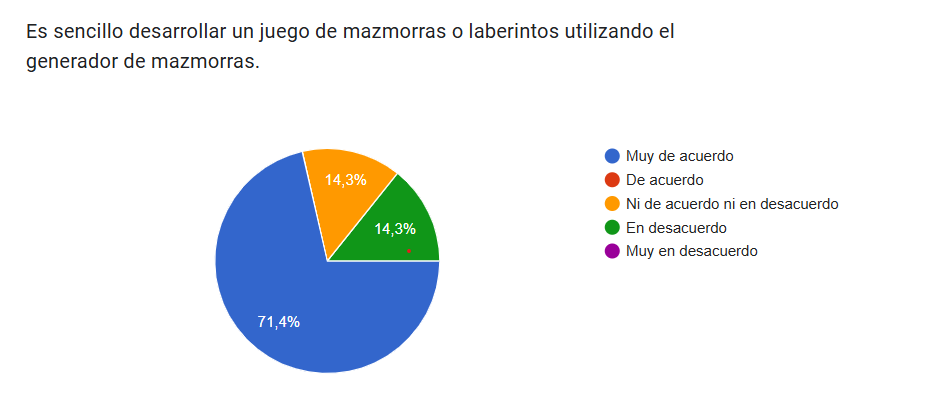
\includegraphics[width=450px,clip=true]{CUESTIONARIO_14.png}
  \caption{Encuesta sobre la facilidad de uso del sistema de mazmorras.}
  \label{fig:CUESTIONARIO_14trucado}
\end{figure}
\raggedbottom

Es relevante mencionar que a excepción del componente de sacudida de cámara, para el cual un 14\% (dos personas) (Figura \ref{fig:CUESTIONARIO_26trucado}) no han estado ni de acuerdo ni en desacuerdo, la totalidad de 
los encuestados están como mínimo parcialmente de acuerdo en que los 'Componentes Independientes' son fáciles de usar y se ajustan a sus respectivos casos de uso.

\begin{figure}[H]
  \centering
  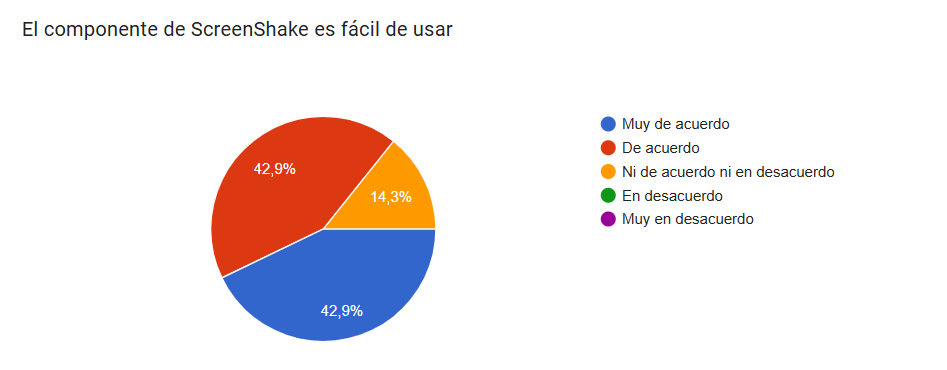
\includegraphics[width=450px,clip=true]{CUESTIONARIO_26.png}
  \caption{Encuesta sobre la facilidad de uso del componente de sacudida de cámara.}
  \label{fig:CUESTIONARIO_26trucado}
\end{figure}
\raggedbottom

La estadística puede parecer menos favorable en las preguntas que suelen hacer mención a la escalabilidad o sencillez del código de la librería, donde un 30\% de los encuestados opina que tanto el sistema de
 diálogo como el de audio son difíciles de escalar (Figuras \ref{fig:CUESTIONARIO_3trucado} y \ref{fig:CUESTIONARIO_6trucado}), o que un 60\% de los encuestados opina que la API del sistema de mazmorras es
  difícil de utilizar (Figura \ref{fig:CUESTIONARIO_15trucado}). Si bien es verdad que esta estadística cobra más sentido al tener en cuenta que el 30\% de los encuestados no tienen un perfil orientado a
   la programación (Figura \ref{fig:CUESTIONARIO_32trucado}), queda otro 30\% de programadores que aún así no opina que la API sea sencilla de utilizar. Una posible explicación al respecto, aparte de que quizás la
   documentación haya sido deficiente al respecto, como se menciona en la figura \ref{fig:tablaFeedback}, es que parte de la API del generador de mazmorras este exige al usuario un cierto
    conocimiento de algoritmos de recorrido de grafos y estructuras de datos complejas, que no todo el mundo, aun teniendo un perfil tecnológico, tiene necesariamente. 

\begin{figure}[H]
  \centering
  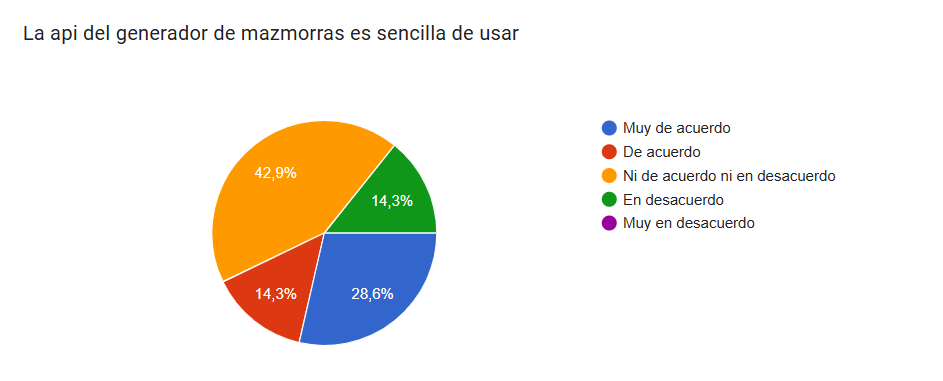
\includegraphics[width=450px,clip=true]{CUESTIONARIO_15.png}
  \caption{Encuesta sobre la sencillez del código del sistema de mazmorras.}
  \label{fig:CUESTIONARIO_15trucado}
\end{figure}
\raggedbottom

\begin{figure}[H]
  \centering
  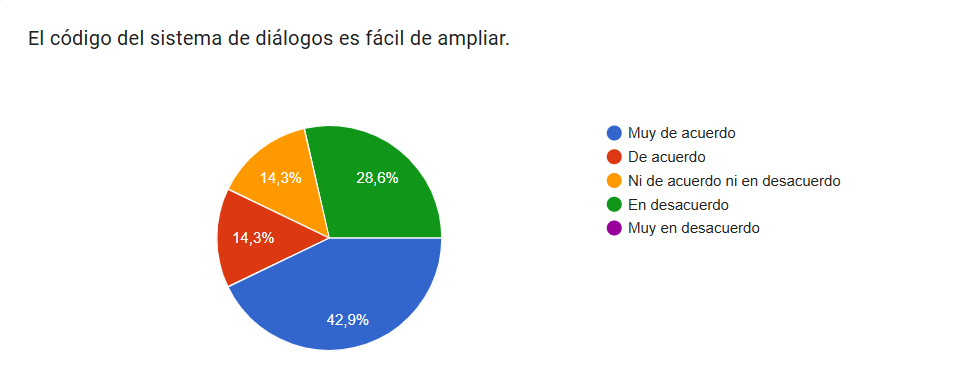
\includegraphics[width=450px,clip=true]{CUESTIONARIO_3.png}
  \caption{Encuesta sobre la escalabilidad del sistema de diálogo.}
  \label{fig:CUESTIONARIO_3trucado}
\end{figure}
\raggedbottom

\begin{figure}[H]
  \centering
  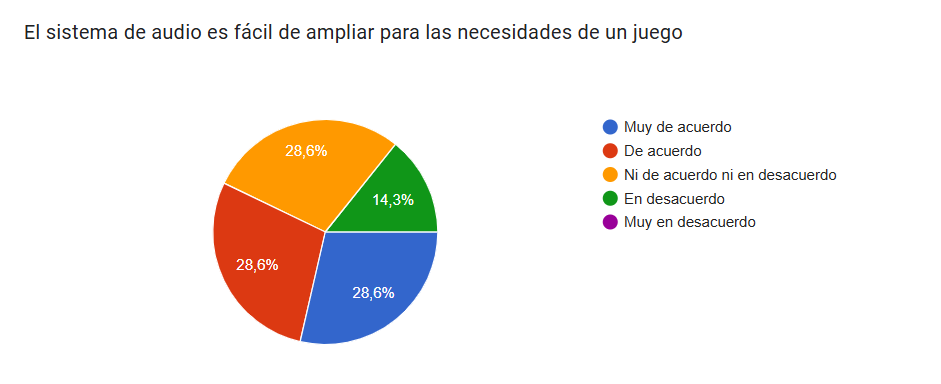
\includegraphics[width=450px,clip=true]{CUESTIONARIO_6.png}
  \caption{Encuesta sobre la escalabilidad del sistema de audio.}
  \label{fig:CUESTIONARIO_6trucado}
\end{figure}
\raggedbottom

\begin{figure}[H]
  \centering
  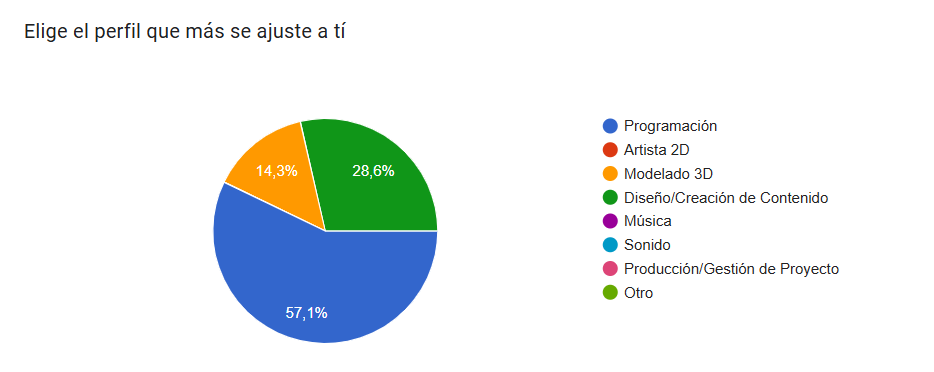
\includegraphics[width=450px,clip=true]{CUESTIONARIO_32.png}
  \caption{Encuesta sobre el perfil del encuestado.}
  \label{fig:CUESTIONARIO_32trucado}
\end{figure}
\raggedbottom

Como pequeños apuntes generales:
\begin{itemize}
    \item La gran mayoría de los encuestados opina que los componentes de movimiento y debug son útiles y efectivos.
    \item La media de edad de los encuestados ronda los veintiséis años de edad.
    \item Un 60\% de los encuestados tienen un perfil técnico, mientras que hay cuatro diseñadores y dos modeladores.
\end{itemize}

\section{Datos Cualitativos}
Hay que hacer énfasis en lo increíblemente participativos que se han mostrado los encuestados a la hora de trabajar en sus propios proyectos, todos los encuestados han usado la gran mayoría de sistemas que ofrecen
los distintos componentes de la libería, por enumerar ejemplos en los dos proyectos ya citados:
\begin{compactitem}
    \item Los niveles de cafetería en Co-Fi Space utilizan el sistema de experiencia.
    \item El movimiento en Co-Fi Space utiliza el componente de movimiento en tercera persona.
    \item El audio tanto en Co-Fi Space como en EcoRescue es gestionado por el sistema de audio.
    \item Los diálogos en ambos proyectos utilizan el sistema de diálogo.
    \item Los iconos de input y los componentes 2D de ambos proyectos utilizan los componentes de Floater y LookAtCamera.
    \item La cuadrícula de EcoRescue utiliza una versión modificada del componente SnapToGrid. 
\end{compactitem}

En cuanto al feedback proporcionado en la encuesta (Figura \ref{fig:tablaFeedback}), ya se ha mencionado que uno de los encuestados opinaba que la documentación es 'mejorable' y que otro de los encuestados opinaba 
que 'el generador de mazmorras es ligeramente complejo de usar sin un trasfondo ténico'. En esta útlima opinión parece estar de acuerdo otro encuestado, que mencionaba que 'algunas de las funcionalidades de la
 librería está muy orientadas a programadores, cosas como ampliar las animaciones de texto no son viables para alguien sin (o con pocos) conocimientos técnicos', sin embargo, tanto ese mismo encuestado como otros 
 cuantos más, coinciden en que 'en cuanto a las funcionalidades que no requieren programar, la librería resulta muy útil y dinámica para prototipar', que es una 'gran librería' y que 'lo demás (lo que no requiere
 implicación técnica) está muy guay'. Uno de los programadores añade incluso que desde el punto de vista técnico 'el código está muy bien comentado y es, por lo general, fácil de leer. Cabe destacar que el sistema de diálogo ha recibido buen feedback, este último programador opina que 'es sorprendente lo cómodo que se hace utilizar el sistema de diálogo', cosa que queda reflejada también
  en los resultados de las encuestas (Figuras \ref{fig:CUESTIONARIO_1} y \ref{fig:CUESTIONARIO_2}). El último punto de feedback indica que sería interesante que 'el componente SnapToGrid fuese aplicable al gameplay'
  esto es algo que, como se ha dicho en la lista anterior, ya se implementó para el videojuego EcoRescue, con lo cual la solución sería tan sencila como implementar los cambios que se ejecutaron para ese proyecto.

En cuanto a resultados tangibles del proyecto, es relevante mencionar que los dos proyectos formales que han sido desarrollados con esta librería han resultado rotundos éxitos. Co-Fi Space obtuvo una sexta posición en 
la 'Game Jam' para la que fue presentado, y el trabajo de fin de grado EcoRescue obtuvo una calificación de nueve con ocho. 
